\section{Micro Processing Unit}
Denne sektion kommer omkring de forskellige moduler, som mikroprocessoren håndterer, samt hvilket styresystem der anvendes.

\subsection{Operativ System}
Når der skal skiftes mellem flere tasks som en processor skal udføre, er det vigtigt at kunne skifte mellem dem på en fornuftig måde; Dette udføres ved hjælp af en schedulerings algoritme. Når der skal implementeres en schedulerings algoritme skal det overvejes hvorvidt det er nødvendigt at lave én designet specielt til projektet, eller om der en en eksisterende der er i stand til at udføre opgaven tilstrækkeligt. I dette project har vi to muligheder til rådighed: FreeRTOS\cite{FreeRTOSorg} og en Run To Complete Scheduler (RTCS).

\subsubsection{FreeRTOS}

FreeRTOS \cite{FreeRTOSorg} er et realtids operativsystem (RTOS), der er en standard løsning som bliver brugt i en mikroprocessor. FreeRTOS giver tilføjer muligheden for at bruge præemptiv skedulering, hvilket vil sige at CPU'en kan stoppe den nuværende task, og køre en eventuelt vigtigere task og derefter vende tilbage til forrige task senere. Hvornår der skal skiftes tasks bliver styret ud fra hvilken prioritet task'en har, eller om der en anden task, der får et interrupt, som CPU'en skal holde øje med.
\\
Udover dette er der er mulighed for at oprette køer, som vil blive nævnt som queues. Disse queues kan der sendes events og data til ved hjælp af en funktion der hedder xQueueSend. 
\\
FreeRTOS kan oprette semaforer, som gør det muligt at flere tasks skal kunne tilgå samme queues, disse semaforer gør at kun en task har adgang til queue'en ad gangen indtil semaforen bliver frigjort igen. For at undgå at styre systemet ikke bliver fastlåst i denne semafor for evigt indsættes der en tid, den kan holde semaforen.
\\
Queues og semaforer bliver oprettet af hhv. xQueueHandle og xSemaphoreHandle. Hvorefter de bliver oprettet ved hjælp af xQueueCreate og xSemaphoreCreateMutex. For at bruge xQueueCreate skal der også bruges længden af queue'en og hvilken parameter den skal indeholde.
\\

\subsubsection{RTCS}

Run To Complete Scheduler (RTCS) er et andet operativ system. RTCS kører som en non preemtiv skedulering, hvilket vil sige at lige så snart CPU'en har forbindelse til en proces/task, så kan den ikke stoppes. I dette system kan der også oprettes queue's.
\\
RTCS har samtidig mulighed for at oprette semaforer, som gør at det er kun en task som kan have adgang til en queue. For at tilføje data til en queue skal funktionen put\textunderscore queue kaldes. Funktionen wait\textunderscore sem bruges til at tilføje en semafor til den specifikke queue.

\subsubsection{Valg af Operativsystem}

Hvis de 2 diskuterede operativ systemer sammenlignes, ses det at RTCS er nemmere at implementere da det ikke er et indviklet styresystem, RTCS tilbyder dog ikke samme sikkerheds udvidelser som freeRTOS gør. Den største begrundelse for at freeRTOS er valgt til dette projekt er at der er implementeret preemptiv skedulering. Dette gøre det muligt, hvis der kommer et vigtigt interrupt, at operativ systemet kan tage CPU'ens nuværende proces og skifte ud med en anden måske vigtigere proces.

\subsection{Tasks}

Der er blevet lavet et task diagram(se figur \ref{fig:task1}, \ref{fig:task2} og \ref{fig:task3}) under udviklingen af programmet til MPU'en. Kommunikation mellem tasks foregår gennem både queues og Shared State Memory. Shared state memory benyttes når der skal sendes data i form af ændring af variabler mellem tasks, mens queues benyttes til at sende beskeder i form af events eller data. Denne metode blev valgt fordi opstår situationer hvor flere tasks skal bruge de samme informationer, og deres eventuelle ændringer af dem påvirker de andre tasks, der skal have kendskab til samme variable.
\\
Af samme årsag benyttes der en semafor til at begrænse adgangen til disse, så der ikke opstår synkroniseringsfejl.
\\
Den centrale task er Menu'en. Denne har til opgave at give brugeren mulighed for manuelt at ændre variabler, såsom tid og position, samt at starte og stoppe kontrolsystemet, og at kommunikere tilbage gennem UART transmit. De tasks som er bygget op omkring denne kan ses i figur \ref{fig:task1}.
\\
Da der er flere forskellige tasks, som skal have adgang til de samme værdier der bliver sat af UART bliver værdierne placeret i shared state memory, som det ses på figur \ref{fig:task2}.
\\
Display task'en holder selvsigende styr på hvad der skal vises, som den får besked om fra Menu'en. Denne får input fra keypad'en og drehimpulsgeberen, der dikterer hvad den skal give videre til LCD.
\\
Geber og Keypad tasksne holder styr på hver deres input, og sender resultaterne i en fælles indgangs kø til Menu'en.
\\
Control systemet tager med jævne mellemrum variabler fra Shared State Memory, og benytter disse til at opdatere det mål pan/tilt-systemet går efter. Den kommunikerer så frem og tilbage med SPI-task'en, som kommunikerer med vores FPGA. Task diagrammet for denne kan ses i figur \ref{fig:task3}.
\\
Årsagen til at dette layout er blevet valgt er at det vurderes at kontrolsystemet ikke skal være afhængig af input fra Menu'en, så det ikke er nødvendigt at benytte menuen til at give den nye koordinater. Ved at separerer den fra Menuen er det muligt for den at køre selvstændigt, uden at den yderligere skal checke en kø for nye koordinater hele tiden.

\begin{figure}[ht]
			\begin{center}
	\includegraphics[width=0.99\textwidth]{Billeder/Taskdiagram1.png}
			\end{center}
	\caption{Task diagrammet over de dele af systemet der centreres over menu'en. Der gives input til UI task'en som så videre giver information hvor der er brug for det, i dette tilfælde Display task'en, Shared State Memory og UART transmit.}
	\label{fig:task1}
\end{figure}

\begin{figure}[ht]
			\begin{center}
\includegraphics[width=0.99\textwidth]{Billeder/Taskdiagram2.png}
			\end{center}
	\caption{Task diagrammet over UART receive. Informationen gemmes i Shared State Memory.}
	\label{fig:task2}
\end{figure}

\begin{figure}[ht]
			\begin{center}
\includegraphics[width=0.99\textwidth]{Billeder/Taskdiagram3.png}
			\end{center}
	\caption{Task diagrammet over kontrol systemet. De værdier den skal bruge kommer fra SPI task'en og eller fra Shared State Memory.}
	\label{fig:task3}
\end{figure}

\subsubsection{Menu}

Den centrale task i systemet er det menu styrede UI-system. Denne har primært til opgave at give brugeren mulighed for manuelt at justere, starte eller stoppe systemet, samt at vise vigtige oplysninger som eksempelvis nuværende position. Menuen styres med drehimpulsgeber og keypad'et, som begge lægger events ind i dens input kø. Den giver events videre til GUI task'en, som styrer de forskellige menuer og display funktioner.



\subsubsection{Universal Asynchronous Receiver/Transmitter}

UART står for universal asynchronous receiver/transmitter. Dette laver kommunikation mellem to enheder. UART transmitterer data i form af bytes og deler dem op i bits og sender dem. Modtager skal så kunne samle dem sammen igen til bytes for at læse det. Uart har en init() funktion som bliver kaldt en gang hvor alle registre bliver sat op som, f.eks. send og modtag. Der bliver også sat en baud rate, som skal være den samme for sender og modtager.
\\
For at sende data kalder vi funktion uart0\textunderscore putc som tager en karakter som input. Dette kan både være tal og bogstaver. Der er en funktion der hedder uart0\textunderscore rx\textunderscore rdy som venter på at den modtager noget.
\\
For at gøre det nemmere har vi lavet en lille protokol, som skal overholdes før microcontrolleren kan tyde det. I figur \ref{fig:UARTCMD} kan ses en liste over de forskellige commands. Et eks. på en UART kald kunne være \texttt{\char`\\}st1803 , som vil sætte tilt delen til 180,3 grader.

\begin{figure}[ht]
			\begin{center}
			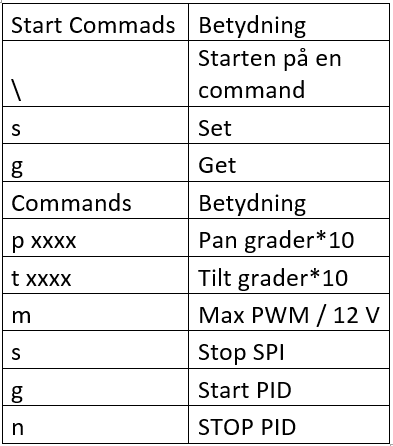
\includegraphics[scale=0.5]{Billeder/UARTCMD.png}
			\end{center}
			\caption{UART commands}
			\label{fig:UARTCMD}
\end{figure}

\subsubsection{Display}

Display task'en tager input fra Menu-task'en og bruger dem til at vælge fra en tabel over prædefinerede billeder, der så sendes til LCD task'en. Disse prædefinerede billeder kan så redigeres hvis der er brug for dette, hvilket er tilfældet hvis der skal vises en dynamisk værdi, som ved show-pan og show-tilt menu-mulighederne.

\subsubsection{LCD}

Den fysiske opsætning af LCD'et kan ses på figur \ref{fig:LCD}, og viser blandt andet at fire databen og R/W benet er forbundet til stel. Med denne opsætning kan man kun skrive til displayet ligesom man er tvunget til at bruge LCD'et i 4-bit mode. Hvis man havde mulighed for at læse fra displayet, kunne man holde øje med et busyflag, der fortæller om LCD'et er optaget, og på den måde sørge for at udnytte displayets tid bedst muligt. Når man kun kan skrive til displayet, er man tvunget til at vente en bestemt tid for at sikre sig at det er klar til at modtage ny data. Til de fleste formål er det dog ikke et problem, at man venter lidt længere end nødvendigt imellem kommandoer. I 4-bit mode kan der kun sendes en nibble ad gangen. For at sende data til displayet, skal dataen skrives ud på de fire databen, derefter flasher man E-benet så LCD'et kan latche og starte behandlingen. RS-benet styrer om den data, der sendes, skal tolkes som data eller en kommando. 

\begin{figure}[ht]
			\begin{center}
			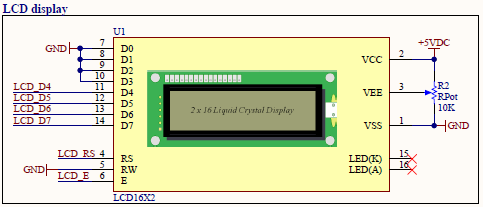
\includegraphics[scale=0.9]{Billeder/LCD.PNG}
			\end{center}
			\caption{LCD pinout}
			\label{fig:LCD}
\end{figure}

Selve LCD-task'en arbejder sammen med resten af systemet ved at afkode et særligt image-format (se figur \ref{fig:LCD_array}), så det vises korrekt på skærmen. Dette image bliver sendt fra display-task'en og indeholder oplysninger om, hvilke karakterer, hvis nogen, der skal skrives til alle 32 synlige adresser på displayet. Udover de 32 karakterer, er der også fire kontrolfelter, som fortæller task'en, hvor cursoren skal placeres efter karaktererne er skrevet ud; om cursoren skal blinke eller bare highlighte nuværende adresse med en streg under karakteren. Det sidste felt bliver sat til at vise adressen, hvor næste karakter skal skrives, når alle 32 karakterer er blevet skrevet første gang. På den måde kan LCD-task'en afgøre om der skal skrives et helt image fra starten, eller bare tilføje en ny karakter til et image der allerede er vist på displayet. Med dette setup kan LCD-task'en finde ud af hvilken ny karakter, der skal tilføjes ud fra den første kontrol-bit, samt hvor cursoren skal placeres efter den er skrevet - hvis den næste adresse, der skal skrives på, er mere end en plads væk, skal cursoren flyttes aktivt. Manipuleringen af images og kontrol-bits foregår i display-task'en - LCD-task'en afkoder bare images, når de bliver tilføjet til dens input-kø.


\begin{figure}[ht]
			\begin{center}
			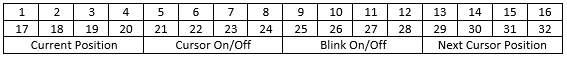
\includegraphics[scale=0.9]{Billeder/LCD_Array.PNG}
			\end{center}
			\caption{LCD Image-format er et array af 36 8-bits størrelser. De første 32 pladser i arrayet repræsenterer de synlige adresser på displayet - de sidste 4 er kontrol-bits.}
			\label{fig:LCD_array}
\end{figure}

\subsubsection{Keypad}

Det udleverede Kit har et tilhørende keypad med 12 knapper fra 0 til 9, samt * og \#. Dette keypad virker som knapper, det er derfor nødvendigt at definere hvad de forskellige knapper skal gøre. For at gøre det simpelt bliver hver knap sat til dens tilsvarende ascii-karakter. Figur \ref{fig:Keypadpins} viser hvordan dens pins er tilsluttet.
\begin{figure}[ht]
	\begin{center}
		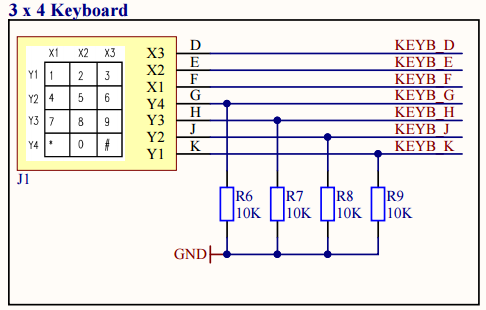
\includegraphics[scale=0.7]{Billeder/Keypadpins.PNG}
	\end{center}
\caption{Keypad pinout}
\label{fig:Keypadpins}
\end{figure}
Den har to porte til knyttet som er PORT A og PORT E. Det betyder at vi kan læse på port E hvis GPIO pinden på port A er aktiv.
\begin{figure}[ht]
	\begin{center}
		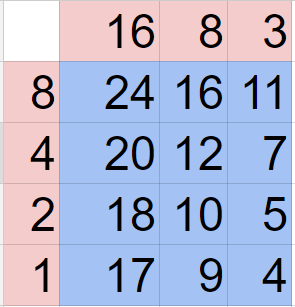
\includegraphics[scale=0.7]{Billeder/keypad.PNG}
	\end{center}
\caption{Giver de fysiske placeringer et tal, som svare et en placering i et array, så som at 1 for placering 24}
\label{fig:Keypad}
\end{figure}


På figur \ref{fig:Keypad} ses de forskellige knappers unikke værdier. Der er til dette oprettet et array hvori placeringerne for hver unik knap er tilføjet, dette ses på figur \ref{fig:Keypad}. For at finde den dertilhørende karakter, findes først x værdierne og derefter y værdierne, herefter kan pladsen i arrayet findes.
\\


\subsubsection{DrehImpulsGeber}

Ved at skrue på drehimpulsgeber kan man inkrementere eller dekrementere en variabel eller sende et event.
Drehimpulsgeberen er en roterende knap som også kan trykkes ned.\\
Drehimpulsgeberen kan sende 30 pulser per rotation.

\begin{figure}[ht]
			\begin{center}
			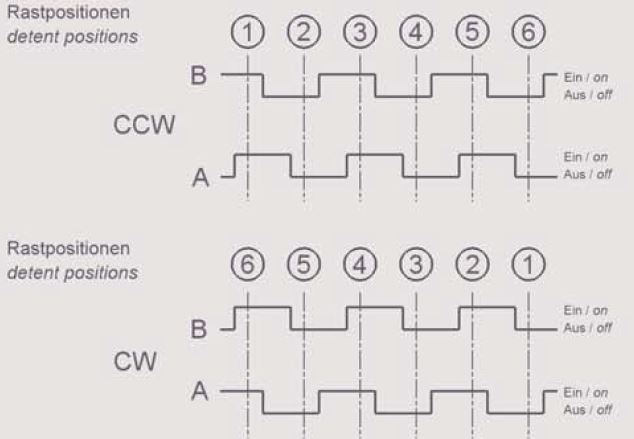
\includegraphics[scale=0.40]{Billeder/DrehImpulsGeber_events.JPG}
			\end{center}
			\caption{Drehimpulsgeber states}
			\label{fig:Impulsgeber}
		\end{figure}

For at finde ud af hvilken retning der bliver skruet på impulsgeberen, kigges der på de tidligere states af impulsgeberen.
eksempelvist hvis der kigges på figur \ref{fig:Impulsgeber} ses det at værdien af B ved henholdsvis en rising eller falling edge på A afhænger af retningen drehimpulsgeberen drejer. Dette bruges til at bestemme hvilket input der skal registeres.


\subsection{Serial Peripheral Interface}
\label{subsec:SPI}

Microcontrolleren (TM4C123GH6PM) der blev udleveret dette semester  indeholder 4 SSI (Synchronous Serial Interface) da disse 4 interfaces alle er ens, med undtagelse af deres pins, er SSI2 blevet valgt som interface, dvs. port B pin 4 er til SSI0Clk (modulets clock), pin 5 er SSI0Fss (frame signalet), pin 6 er SSI0Rx (modtagelse) og pin 7 er SSI0Tx (afsendelse).

Til SSI modulet er der 3 forskellige data formater:

		\begin{figure}[ht]
			\begin{center}
			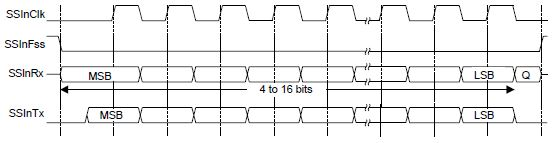
\includegraphics[scale=1]{Billeder/FS_Frame_Format.JPG}
			\end{center}
			\caption{FreeScale Frame Format (Single Transfer)}
			\label{fig:FSFrameFormat}
		\end{figure}
	
Da Freescale kan ses i figur \ref{fig:FSFrameFormat} er den eneste SPI iblandt de tre SSI moduler, og kravet til projektet var at der skulle kommunikeres via SPI, er det det som bliver anvendt.

		\begin{figure}[ht]
			\begin{center}
			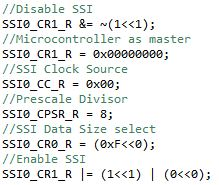
\includegraphics[scale=0.8]{Billeder/SPI_Setup.JPG}
			\end{center}
			\caption{Setup af Freescale SPI}
			\label{fig:SPI_Setup}
		\end{figure}

For at opsætte Freescale, kan ses i figur \ref{fig:SPI_Setup} skal SSI modulet deaktiveres, og så kan MPU'en sættes som master, ved at skrive nul til control registret.
Derefter skal clock configurations registret sættes til 0 så system clocken bruges.
Da der ønskes en 2 Mbps clock bruges ligning \eqref{eq:clock}, som kan findes i \cite{TM4C123GH6PMDatasheet} side 953.

\begin{align}
\begin{split}
2*10^6 bps &= \dfrac{16*10^6 Hz}{CPSDVSR * (1 + 0)}\\
CPSDVSR &= \dfrac{16*10^6 Hz}{2*10^6 bps}\\
CPSDVSR &= 8
\end{split}
\label{eq:clock}
\end{align}

Så sættes kontrol registret for SSI2 til 0xF da bit 3:0 angiver data størrelse, 0xF er så 16-bit data. Samtidig bliver Freescale SPI sat op, da bit 4 og 5 bestemmer frame formatet, og hvis de begge er lave betyder det at Freescale er valgt. 
og igen sættes bit 1 i kontrol registret for SSI1 til høj så SSI'en er aktiveret.

\subsection{PID-Controller}

PID-controllerens opgave består i at beregne sig frem til et passende PWM-signal, til at regulere motoren med, ud fra forskellen imellem motorens ønskede og faktiske position. Dette PWM-signal skal drive fejlen i 0 på en måde, der opfylder projektets designmål. Beregningen er styret af de tre konstanter $K_{P}$, $K_{I}$ og $K_{D}$, som igennem en analyse af systemets opførsel, beregner sig frem til (se afsnit \ref{sec:Controller_Design}). Denne analyse antager et ideelt system, hvor man hele tiden med uendeligt små tidsintervaller kan justere controllerens output. Det er ikke muligt at implementere en controller i den form, så der vil være en forskel på den programmerede og den modellerede controllers opførsel.


\subsubsection{Fundamental funktion}

Selve beregning af outputtet sker ved, at controlleren med jævne mellemrum kigger på set-point'et for en motor, og sammenligner det med motorens faktiske position. Dette giver en fejlværdi, der løbende holdes øje med. 
\begin{itemize}[noitemsep]
	\item For at finde proportionaltermet ganges konstanten $K_{P}$ på fejlværdien
	\item For at finde integraltermet ganges konstanten $K_{I}$ på en løbende summering af arealet under fejlen. Dette areal findes ved at gange $dt$ på fejlen, og så lægge det til hver gang udregningen køres igennem. På figur \ref{fig:Riemann} kan man se, hvordan integralet hele tiden vokser, så længe en fejl er til stede.
	\item For at finde differentialtermet ganges konstanten $K_{D}$ på forskellen imellem den nuværende fejl og den forrige fejl delt med dt. Det svarer til at beregne $\Delta e/\Delta t$.
\end{itemize}

\begin{figure}[ht]
	\begin{center}
	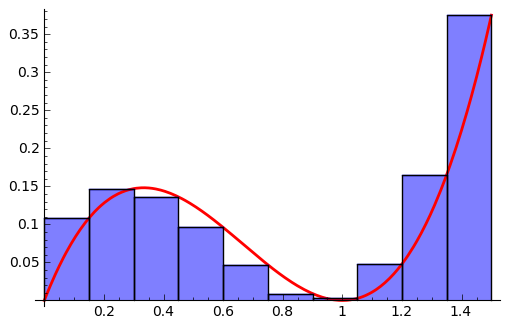
\includegraphics[scale=0.8]{Billeder/RiemannSum.png}
	\end{center}		
	\caption{Her ses en visualisering af det løbende integral der udregnes i starten af hver sample-periode. Arealet dækket af alle de blå bjælker viser størrelsen af integralet, og den røde kurve viser hvordan fejlen ændrer sig over tid.}
	\label{fig:Riemann}
\end{figure}

Når de tre termer er fundet, summeres de for at finde det endelige output fra udregningen. Dette output er i sig selv ikke brugbart til at finde en duty cycle som motoren skal reguleres med. der skal defineres et interval som outputtet kan operere indenfor. På den måde er det muligt, at mappe positionen til en duty cycle mellem 0 og 255 ved at finde ud af hvor outputtet befinder sig i intervallet. På figur \ref{fig:Mapping} ses en visualisering af denne mapping. Hvis outputtet er negativt betyder det at retningen skal ændres på motoren, men det ændrer ikke noget på hvilken duty cycle, der skal sendes i sidste ende.

\begin{wrapfigure}{R}{0.5\textwidth}
	\begin{center}
	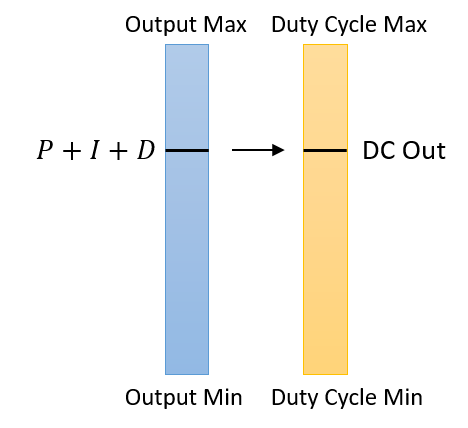
\includegraphics[scale=0.8]{Billeder/Mapping.png}
	\end{center}		
	\caption{Her ses hvordan PID-outputtet mappes til en tilsvarende duty cycle}
	\label{fig:Mapping}	
\end{wrapfigure}
\paragraph{Duty Cycle}

Det har en ret stor betydning hvilke duty cycles der kan sætte som output. Med duty cycles under 15 $\%$ kan motoren, næsten ikke slæbe systemet rundt, og hvis duty cycle er over 75 $\%$ kan systemet justere så voldsomt, at selve platformen som rammerne er monteret på, begynder at flytte sig rundt på bordet grundet en hård opbremsning. Af den grund blev der tilføjet et interval mellem 15 $\%$ og 39 $\%$ som controlleren kunne justere indenfor. For at forhindre systemet i at oscillere omkring set-point'et med en duty cycle på 15 $\%$ låses motoren, når fejlen er 0. Motoren låses når de to in-signaler sættes lave samtidig med at enable er høj.

\paragraph{Skalering af beregninger}

Et problem ved at bruge FreeRTOS som platform er, at det ikke er muligt at regne med floating point tal. MPU'en kan fint arbejde med dem, da den har et floating point unit, men port mappet til FreeRTOS er lavet til en processor der ikke har en. Det giver problemer når FreeRTOS laver kontekst skift. Den kan ikke finde ud af at gemme floats i memory, når der skiftes imellem tasks. Så hvis der benyttes floats, så ender styresystemet i et fault interrupt.

Af den grund er alle udregninger nødt til at foregå på heltal. For at kunne slippe afsted med det, er alle operander i udregningerne nødt til at blive skaleret, da der tit er tale om kommatal i en eller anden størrelsesorden. Den bedste løsning opnåes ved at bruge \textit{fixed point} aritmetik. Det kan dog være svært at tyde tallene, når man læser koden, da de bliver konverteret til en størrelse der ikke, ved første øjekast, har nogen relation til det oprindelige tal. En simplere løsning i samme boldgade, som blev implementeret, er at skalere tallene med størrelsesordner af faktor 10. Det gør tallene ret store, men i kraft af at MPU'en arbejder med 32 bits ad gangen, er der ret højt til loftet. Det er også lettere for normale mennesker at arbejde med decimal tal.

Det er vigtigt at sørge for at alle termerne bliver skaleret lige meget, så forholdet imellem termerne ikke ændres. De to ting der er nødvendige at skalere er $dt$ og gainet til controlleren, da de begge er i størrelsesorden $10^{-3}$. P-termet bliver kun påvirket af gainet, mens både I- og D-termet bliver påvirket af gain og $dt$, men D-termet bliver påvirket af $dt$-skaleringen modsat i forhold til I-termet. Dette betyder at med en skaleringsfaktor på $10^4$, ender med et P-term skaleret med $10^4$, et I-term skaleret med $10^8$ og et D-term skaleret med $10^0$. Det skal der selvfølgelig justeres for, så outputtet giver mening.

\paragraph{Integral Windup}

Et problem med PID-controlleren er integral windup. Integral windup er, når arealet under fejlen vokser sig så stort at I-termet kommer til at dominere outputtet. Det er et stort problem for især langsomme systemer, som bruger lang tid på at drive fejlen i 0. Så længe der er en fejl til stede, vil integralet vokse sig større. Det kan blive så stort at systemet er nødt til, at tilbringe lang tid med en modsatrettet fejl for at komme tilbage til set point; Det er ikke en opførsel man er interesseret i. I de fleste tilfælde er integralets eneste vigtige bidrag at forhindre steady state fejl ved at "trække" systemet på plads, når systemet er tæt på målet. Af den grund er der mange implementeringer der ignorerer integraltermet, når fejlen er over en vis størrelse. En anden mulighed er at sætte et loft på, hvor stort integralet kan blive. Til dette projekt blev begge metoder benyttet, da det viste sig at være problematisk at kontrollere integratoren.

\paragraph{Deadband}

For at kompensere for at systemet har diskrete koordinater, hvilket resulterer i at systemet ofte fortsætter frem og tilbage over den ønskede position, benyttes der et deadband. Denne er implementeret ved at systemet aktiverer en motor bremse hvis der måles at systemet er i den position der ønskes. Dette forhindrer at systemet gentagne gange fortsætter forbi den ønskede position, da deadbandet låser systemet hvis der er så lidt hastighed, at den kan bevæge sig gennem det tick der forsøges at ramme. Såfremt der er så meget hastighed i systemet, at den blot fortsætter igennem bremsen bliver denne blot slået fra igen når systemer kommer ud på den anden side, hvorved controlleren frit kan korrigere for steady state fejl.

\subsubsection{PID Task}

PID task'en har to tilstande: idle og running. I idle-tilstanden ventes der på et \texttt{PID\_START\_EVENT}, der skifter tilstanden til running. I running-tilstanden køres funktionen \texttt{PID\_update()} med faste intervaller. Denne funktion sørger for at hente set point og den fysiske position af rammerne for både pan- og tilt-systemet. Dette kræver kommunikation med SPI-task'en. Kommunikationen er styret fuldstændig af PID-task'en, der bare benytter de services som SPI-task'en tilbyder. Når \texttt{PID\_update()} bliver kaldt, beregnes outputtet for pan-systemet og derefter for tilt-systemet.\\
Når outputtet for hhv pan- og tilt-systemet er beregnet, sendes et \texttt{SET\_PWM\_EVENT} til SPI-task'en som sender informationen videre til FPGA'en. Efter eventet er sendt venter PID-task'en i 5 ms, hvorefter den sender et \texttt{GET\_POS\_EVENT} til SPI-task'en, som henter den nuværende position af både pan- og tilt-systemet fra FPGA'en og gemmer den i shared state memory. Når den er færdig med det, sendes et \texttt{PID\_UPDATE\_EVENT} tilbage til PID-task'en som starter cyklusen forfra. Hele processen kan ses på figur \ref{fig:PID_update}.

\begin{figure}[ht]
	\begin{center}
	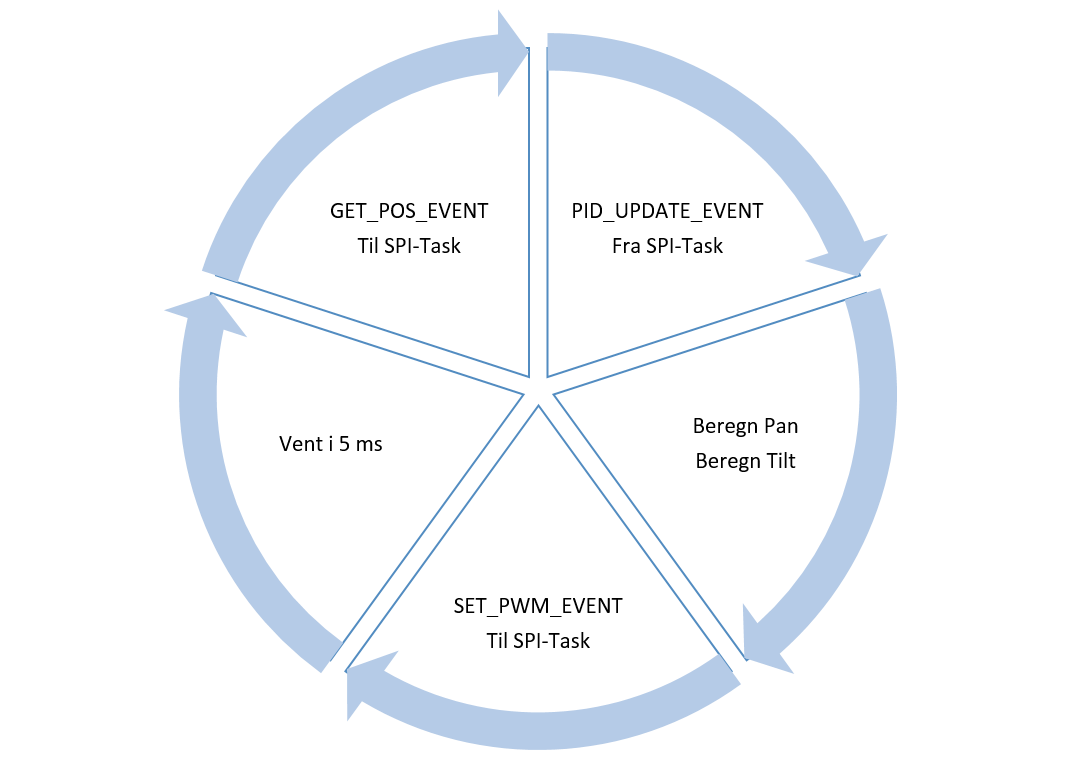
\includegraphics[scale=0.5]{Billeder/PID_update.png}
	\end{center}		
	\caption{Her ses en visualisering af den cyklus som PID-task'en styrer, når den er i running-tilstanden}
	\label{fig:PID_update}
\end{figure}

\paragraph{Filter}
En alternativ måde at gribe implementeringen an på, er at lave controlleren som et filter. Det kan lade sig gøre ved at mappe overføringsfunktionen over i z-domænet og på den måde finde filterkoefficienterne. Denne metodik tillader implementeringen af andre controller-typer som fx lead- og lag-controllere, da lettere man kan implementerer flere slags overføringsfunktioner. Dette blev ikke udforsket, da den anden måde som udgangspunkt virkede simplere, samt at dette ikke ville øge præcisionen af vores system, hvilket var vores første prioritet.

\subsubsection{Delkonklusion}
PID-controllleren blev implementeret med en sample frekvens på 200 Hz fordi freeRTOS som standard ikke kunne vente i kortere intervaller uden ekstra funktionalitet man selv tilføjer. Dette er endnu en faktor, der gør at implementeringen ikke helt præcist  afspejler den modellerede controller. For at forhindre oscillationer omkring set point benyttes et deadband hvor motoren låses når fejlen er 0. 

%Der kunne også have været brugt \textit{fixed point} aritmetik til udregningerne på microcontrolleren, men det blev vurderet at det skabte flere problemer end det løste under udviklingen. Det er noget som kunne tages op igen på et senere tidspunkt. For at slippe af med integral windup blev der sat et loft på hvor stort integralet kunne blive, og det blev slet ikke brugt, når fejlen var over en bestemt størrelse.  En filterimplementering blev ikke udforsket, men kunne helt klart være en mulig forbedring af systemet i fremtiden. XXXX Gør den stadig det?

\subsection{Koordinat oversættelse}

\label{subsec:koordinat}

Pan og tilt rammen har en præcision på en tredjedel grad, og da det samtidigt er et primært krav at denne skal kunne fungere med input i form af sfæriske koordinater, er det nødvendigt at have en koordinat oversættelse fra de horizontale koordinater, til sfæriske koordinater. se figur \ref{fig:Horizontal}. Denne oversættelse skal tage højde for de fysiske begrænsninger systemet har. Oversættelsen skal derfor lave en oversættelse i pan delen der afspejler at denne kun kan bevæge sig lidt over 180 grader uden at der opstår problemer med de ledninger der styrer tilt delen. Dette er dog slet ikke nok til at lave et effektivt teleskop system.
\begin{figure}[!h]
	\begin{center}
		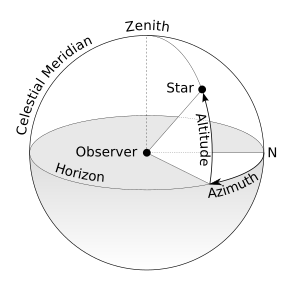
\includegraphics[width=0.5\textwidth]{Billeder/Horizontal.png}
	\end{center}		
	\caption{Her ses hvordan det horizontale koordinat system fungerer}
	\label{fig:Horizontal}
\end{figure}

Mens pan delen kun har 180 graders frihed har tilt delen fuld frihed. Dette betyder at vi kan udnytte denne til at tilgås det område som pan delen ikke kan tilgå. Dette gøres ved blot at spejle tilt delen omkring origo, dette kan ses på figur \ref{fig:tilt_spejl} samtidig er figur \ref{fig:tilt_spejl} den spejlede version af figur \ref{fig:tilt_spejl1}. Nulpunktet for pan- og tilt-systemet er lokeret som på figur \ref{fig:Nulpunkt}. 

\begin{figure}[!h]
    \centering
    \begin{subfigure}[b]{0.3\textwidth}
       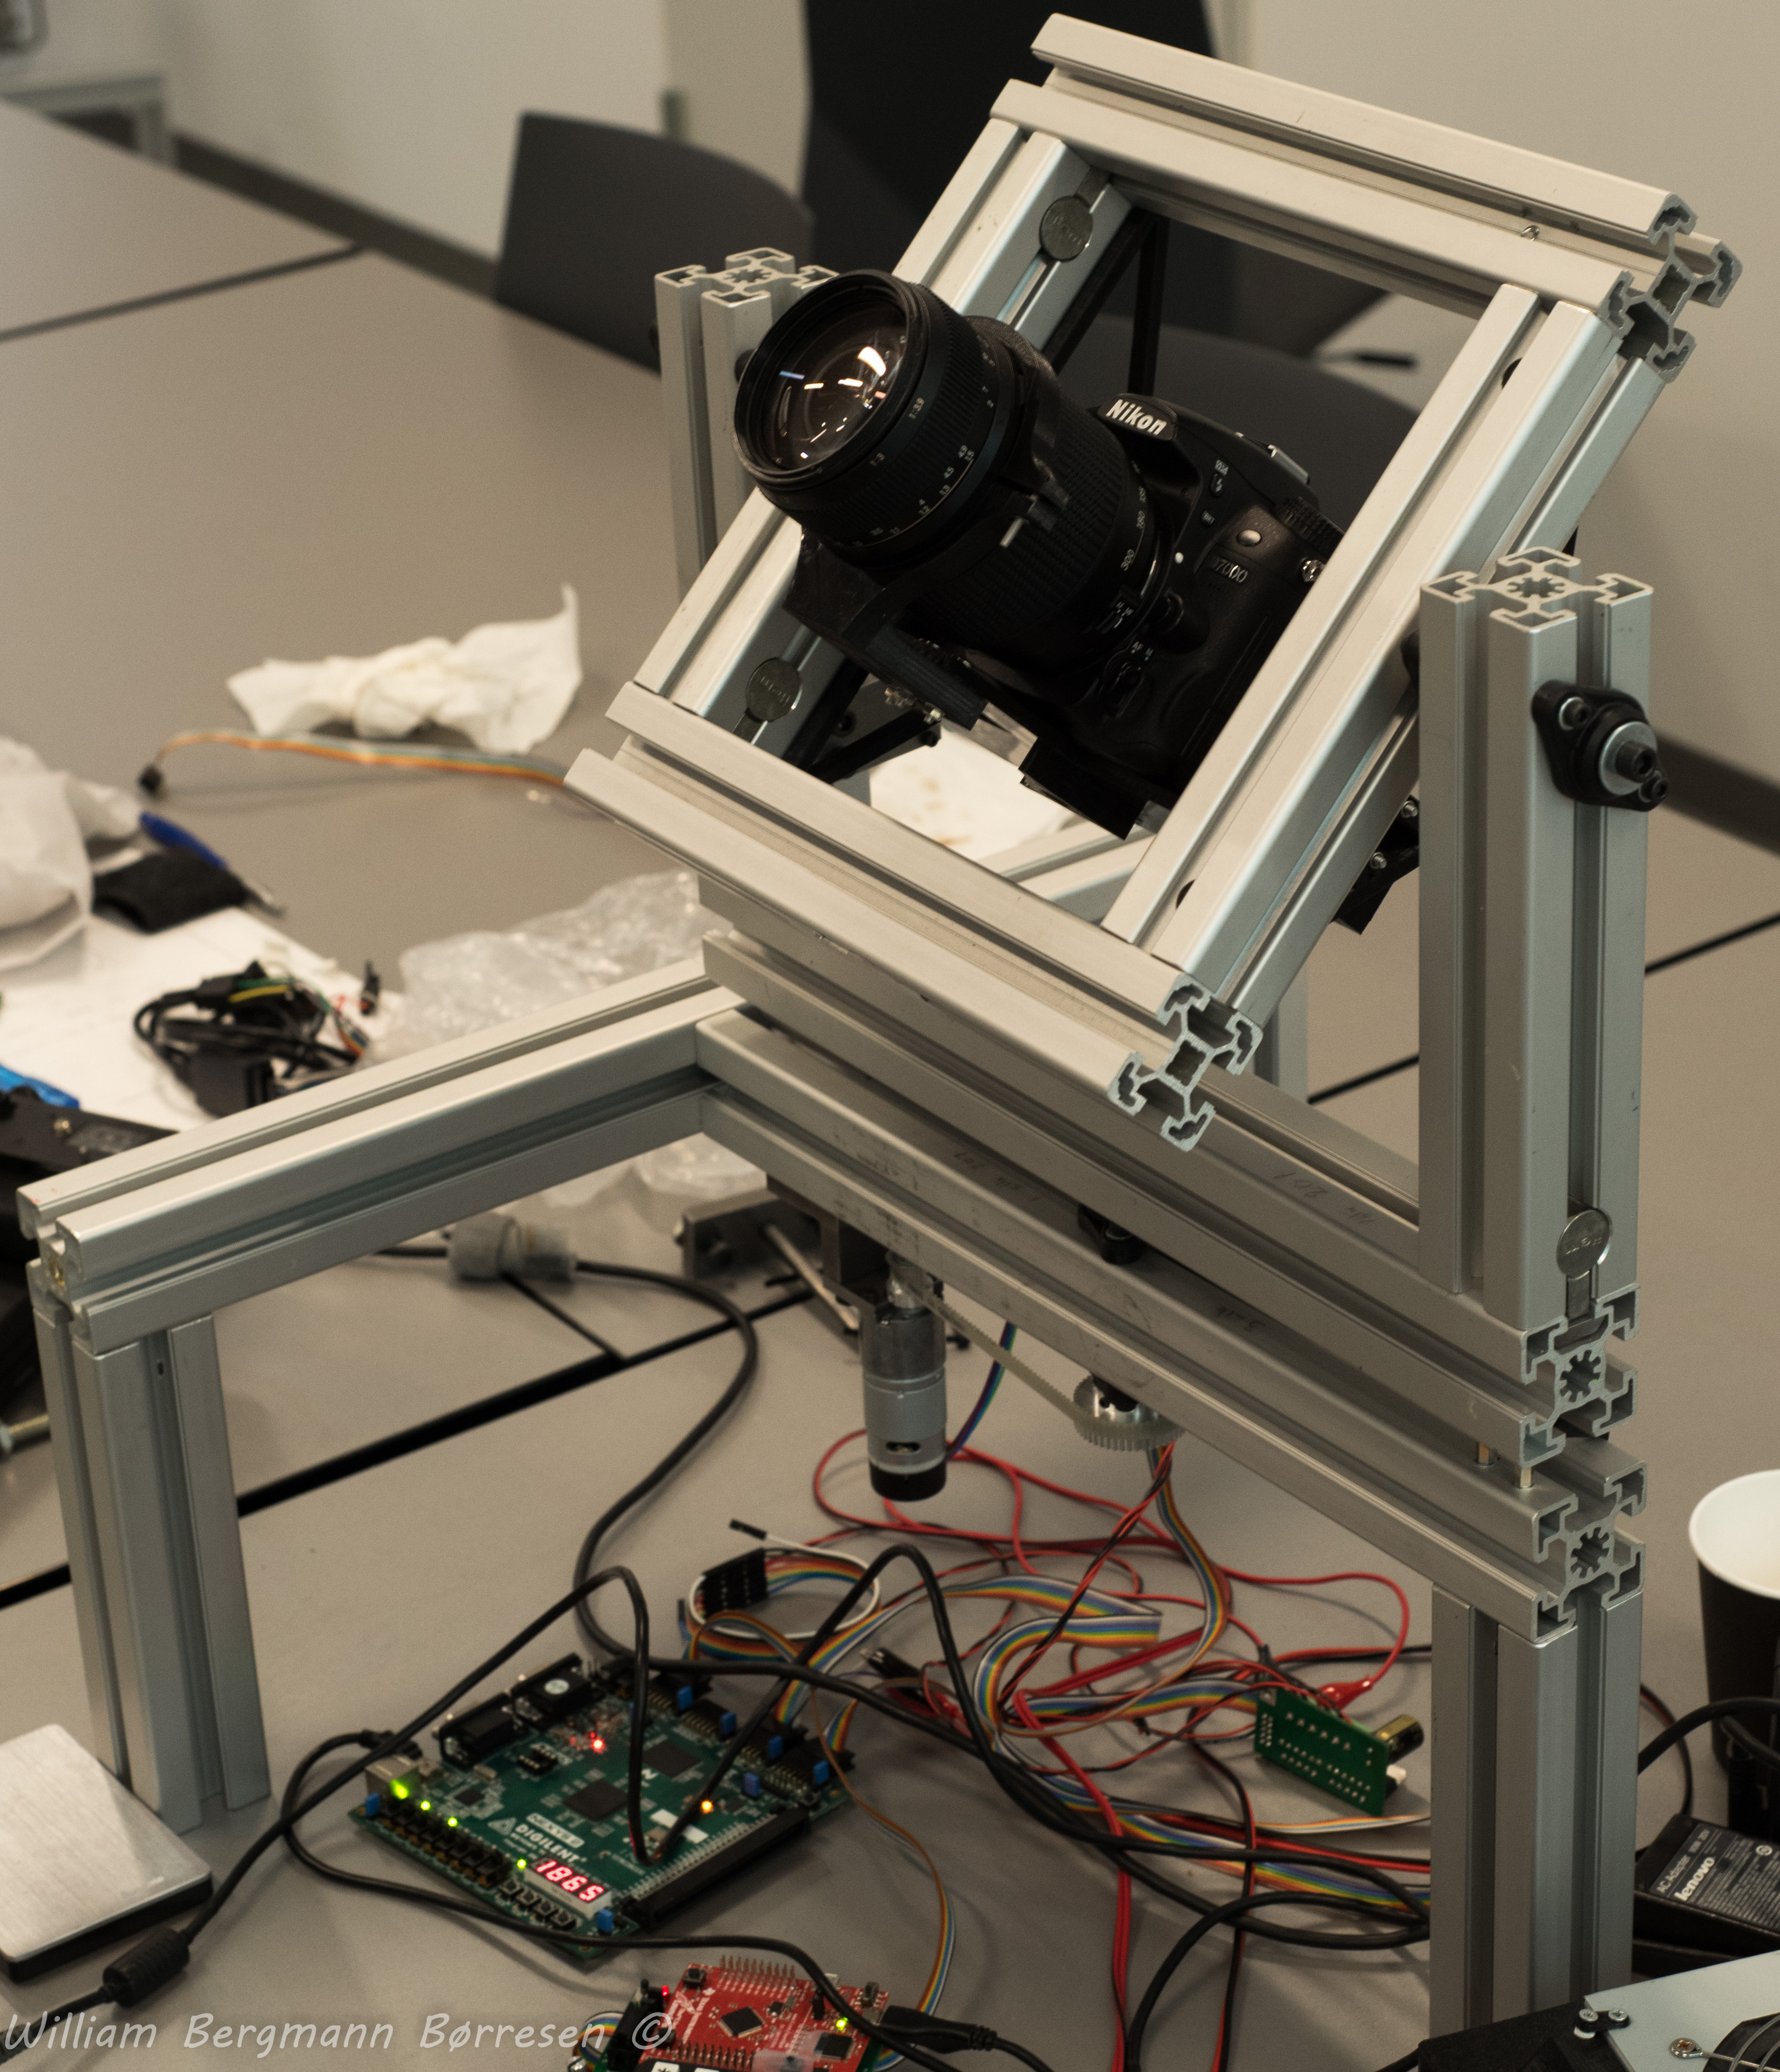
\includegraphics[width=1\textwidth]{Billeder/Tilt45deg.jpg}
        \caption{}
        \label{fig:tilt_spejl1}
    \end{subfigure}
  \begin{subfigure}[b]{0.3\textwidth}
        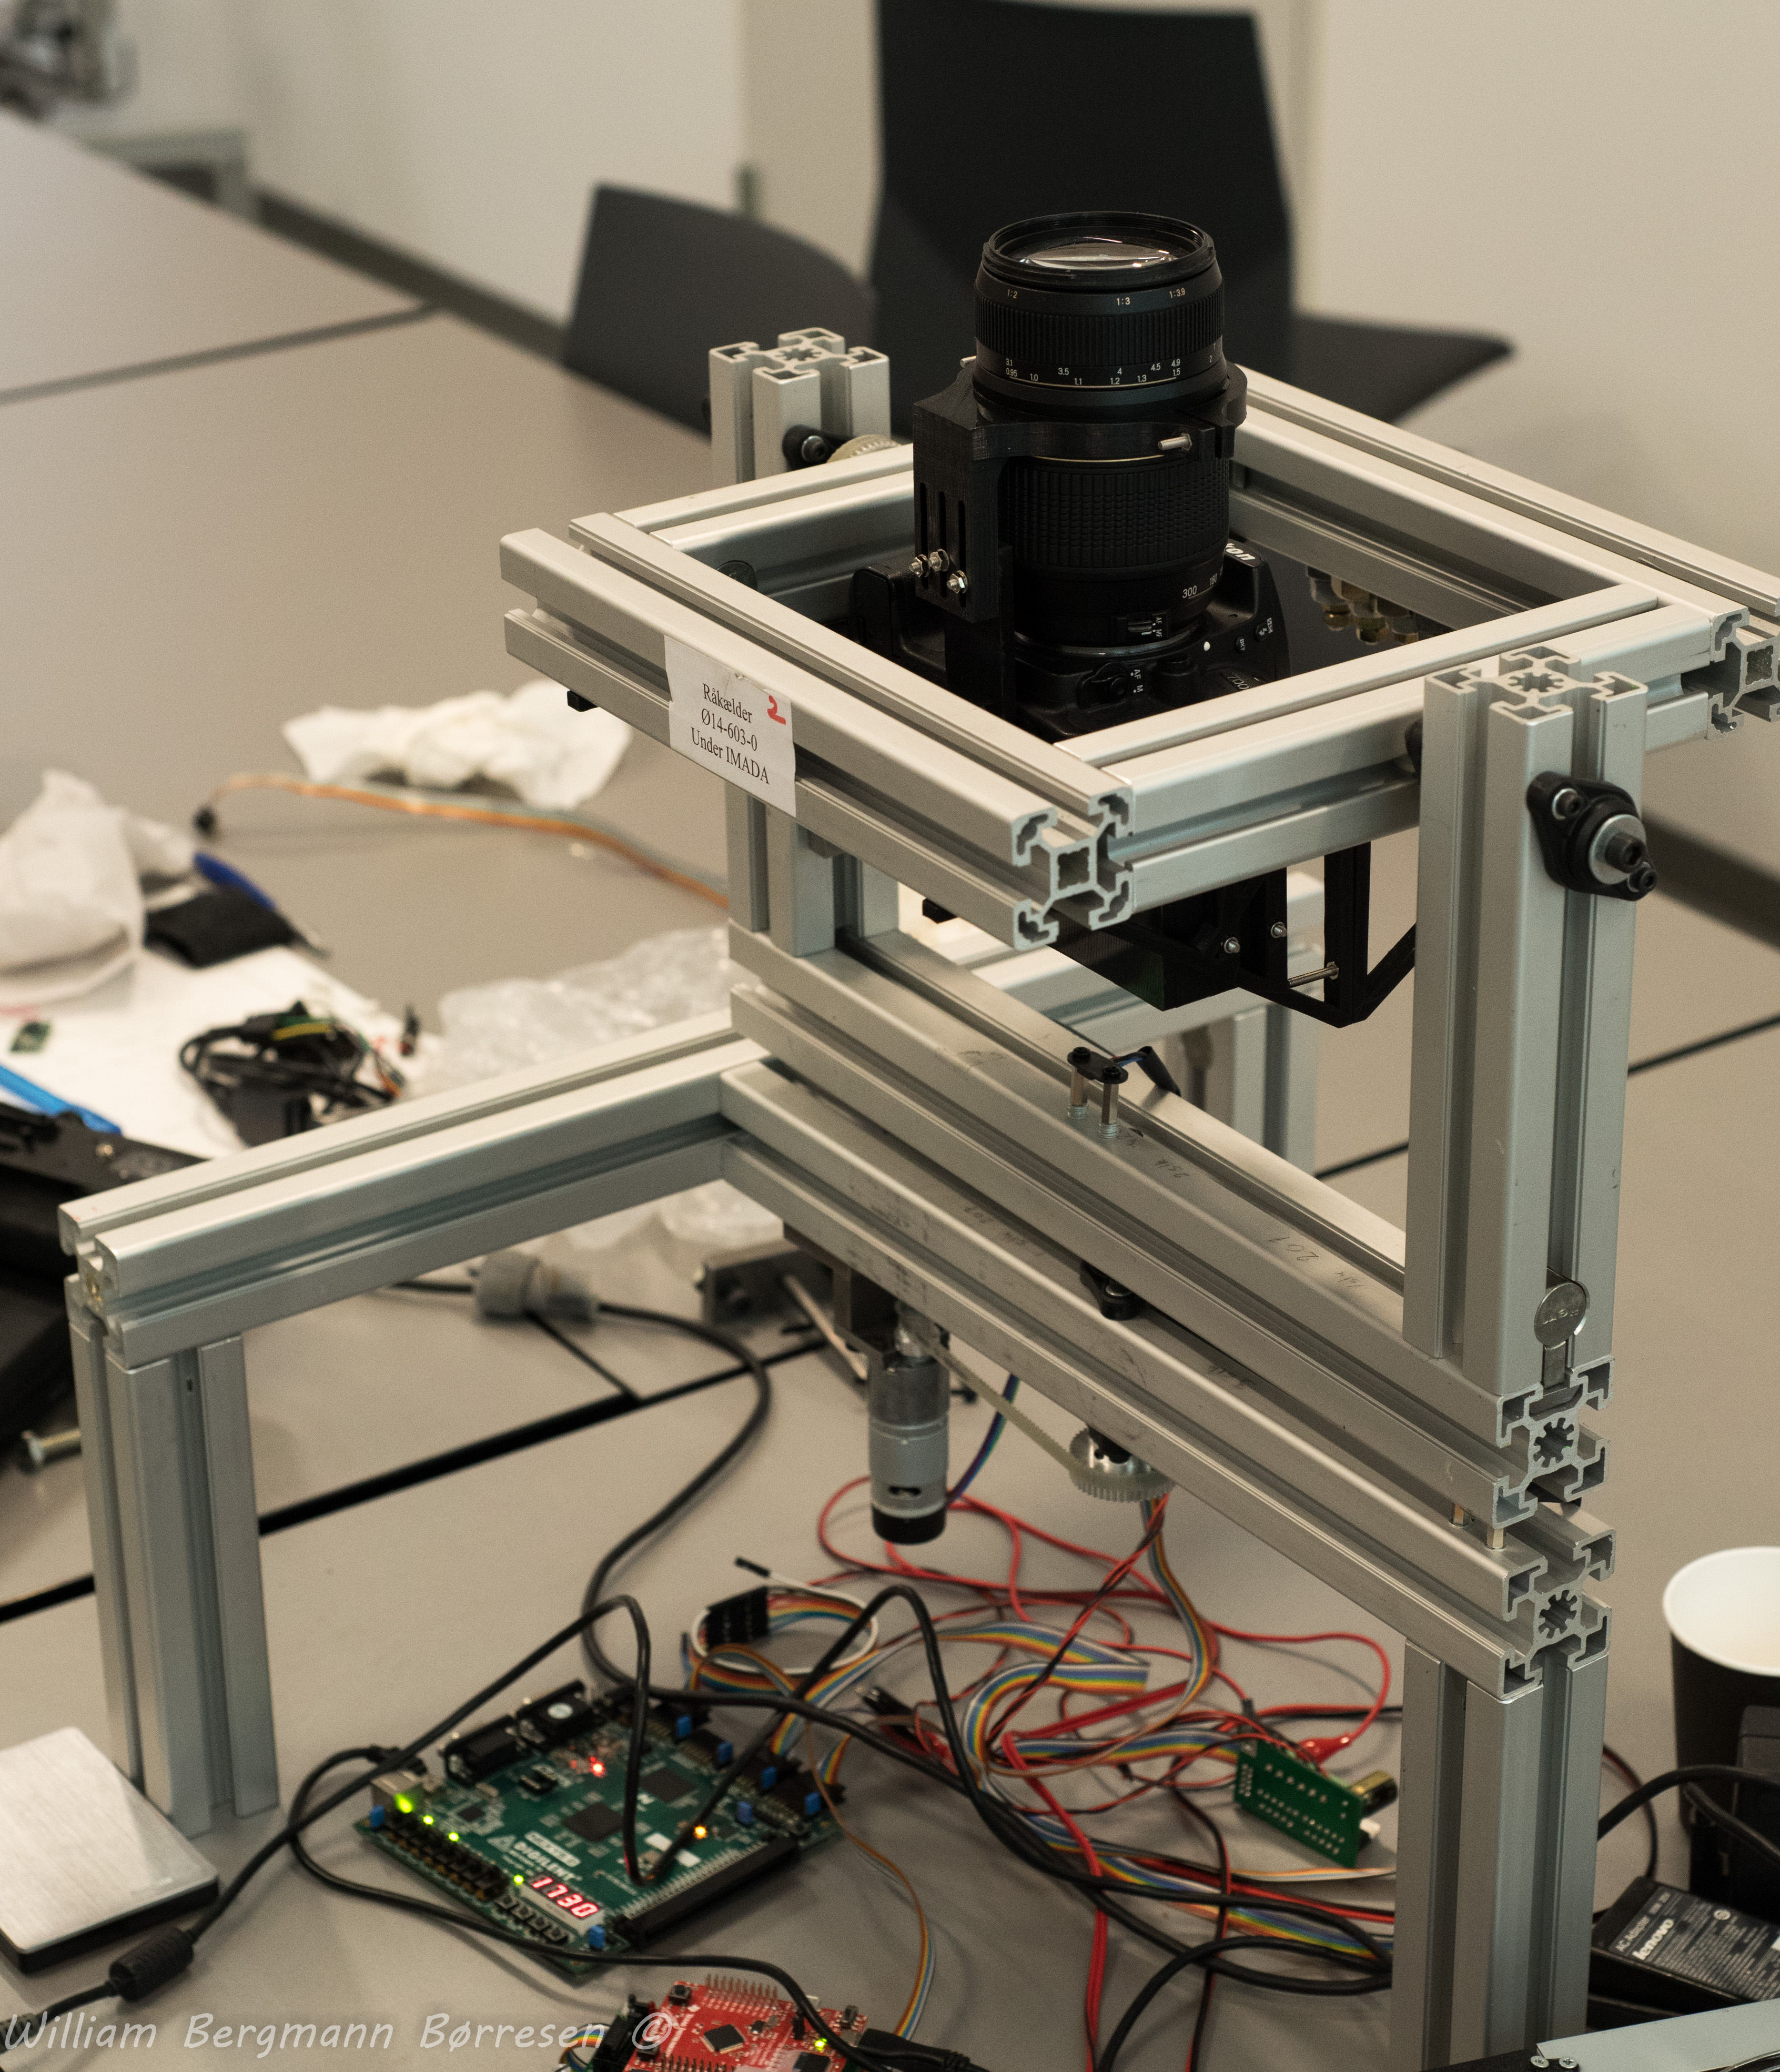
\includegraphics[width=1\textwidth]{Billeder/Nulpunkt.jpg}
        \caption{}
        \label{fig:Nulpunkt}
    \end{subfigure}
    \begin{subfigure}[b]{0.3\textwidth}
        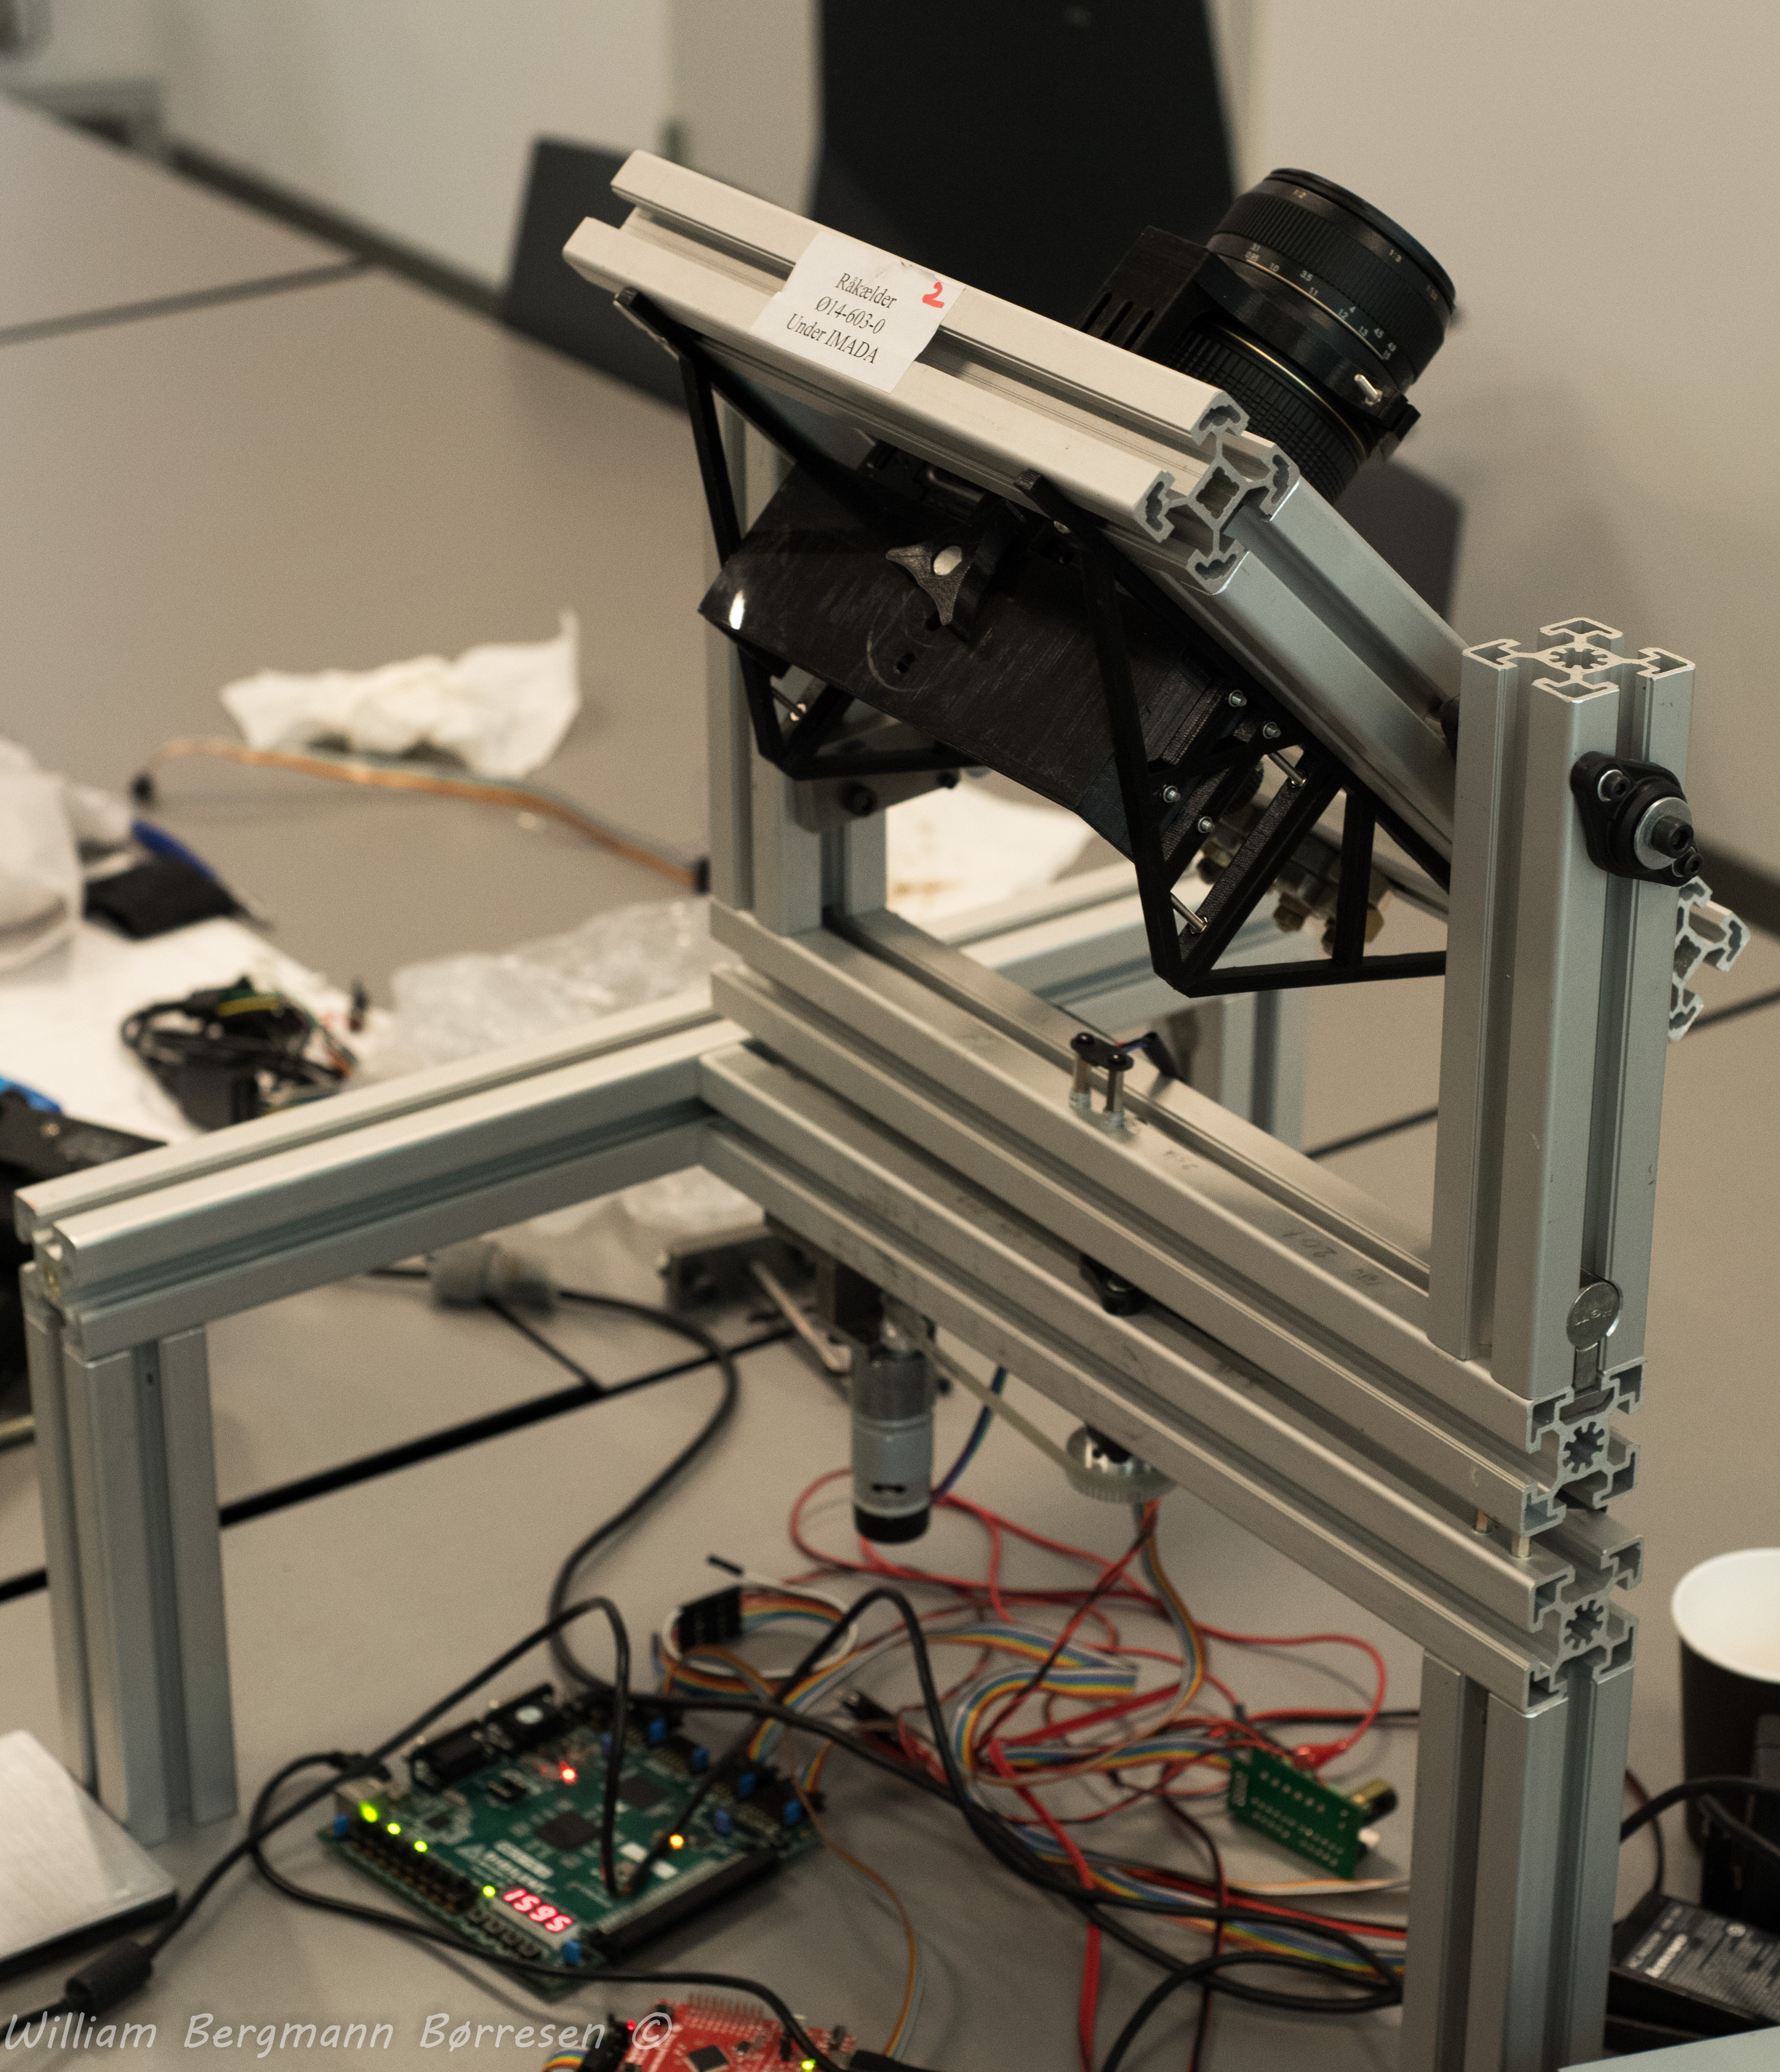
\includegraphics[width=1\textwidth]{Billeder/Tilt315deg.jpg}
        \caption{}
        \label{fig:tilt_spejl}
    \end{subfigure}
   \caption{Her demonstreres hvordan en spejling foregår. Til venstre ses systemet i position pan: 0$^{\circ}$ tilt: 45$^{\circ}$, i midten ses origo ved pan: 0$^{\circ}$, tilt: 0$^{\circ}$, og til højre ses hvad der sker når vi forsøger at bevæge systemet over i det område som pan-systemet ikke kan komme over i, ved pan: 180$^{\circ}$, tilt: 45$^{\circ}$.}
\end{figure}

Denne position, som kan ses på figur \ref{fig:Nulpunkt}, er valgt fordi den passer bedst overens med det sfæriske koordinat system, som kan ses på figur \ref{fig:Spherical}. Alternativt kan pan delens nulpunkt placeres således at den har sit nulpunkt i kanten af dens bevægelsesområde, men dette blev fravalgt da den sensor der benyttes til at indstille systemet ligger på denne position. Grunden til at dette ikke er gjort for tilt-systemet ,er at den valgte retning både gør det nemmere at spejle det omkring origo, samtidig med at det passer bedre med det sfæriske koordinat system.

\begin{figure}[!hb]
	\begin{center}
		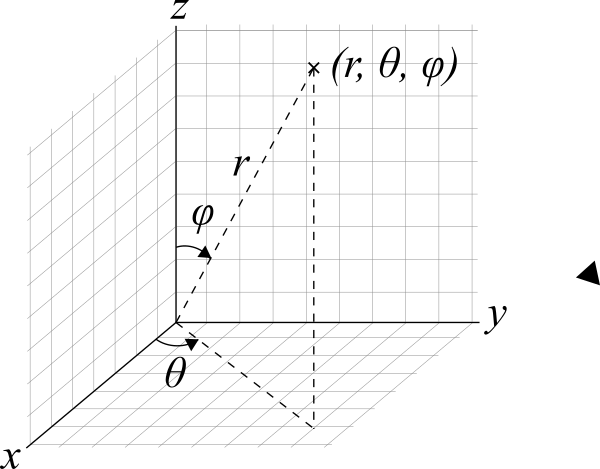
\includegraphics[width=0.5\textwidth]{Billeder/Spherical.png}
	\end{center}		
	\caption{Her ses hvordan det valgte sfæriske koordinat system fungerer. Der er flere mulige baser for sfæriske koordinater, men dette er det mest matematisk rigtige, hvilket er grunden til at dette blev valgt.}
	\label{fig:Spherical}
\end{figure}
En stor fordel ved denne koordinat oversættelse er at den eliminerer nødvendigheden for et sikkerhedssystem på MPU'en. Dette er naturligt en del af koordinat oversættelsen, da alt mellem 90 og 270 grader på pan systemet, som er det områder hvor der kan ske mekaniske skader, slet ikke er aktuelt, på grund af spejlingen af koordinaterne. Det skal dog noteres at dette ikke eliminerer behovet for et sikkerhedssystem på FPGA'en, som der stadig er brug for i tilfælde af der forekommer problemer med MPU'en, så som en løs forbindelse, en fejl der får hele MPU'en til at fryse, bælter som kammer over, eller overshoot der går ud over den sikkerheds grænse, som er blevet besluttet.




















